\documentclass[a4paper,12pt]{article}
\usepackage[utf8]{inputenc}
\usepackage[russian]{babel}
\usepackage{graphicx}
\usepackage{amsmath, amssymb}
\usepackage{algorithm2e}
\usepackage{hyperref}
\usepackage{subcaption}
\usepackage{dirtree}
\usepackage{booktabs}

\title{\textbf{Оптимизация методом Spider Wasp Optimizer (SWO)}}
\author{Кривнюк Константин}
\date{гр. 9302}


\begin{document}

\maketitle

\begin{abstract}
В данном реферате представлен алгоритм Spider Wasp Optimizer (SWO), вдохновленный охотничьим поведением пауков-ос. Рассматривается структура проекта, основные этапы алгоритма и его применение к оптимизационным задачам. Приведены псевдокод алгоритма, тестовые функции и результаты сходимости.
\end{abstract}

\tableofcontents

\newpage

\section{Введение}
Spider Wasp Optimizer (SWO) — это инновационный метаэвристический алгоритм, имитирующий охотничьи и спаривательные стратегии пауков-ос. Его ключевые преимущества — высокая эффективность в глобальной оптимизации и гибкость для широкого класса задач.

Цель данного проекта — разработать реализацию SWO, протестировать алгоритм на стандартных тестовых функциях и проанализировать его сходимость.

\newpage

\section{Структура проекта}
Проект имеет следующую структуру:

\dirtree{%
.1 report.
.2 images.
.2 report.pdf.
.2 report.tex.
.1 sw\_optimizer.
.2 \_\_init\_\_.py.
.2 sw\_optimizer.py.
.1 test\_functions.
.2 \_\_init\_\_.py.
.2 ackley.py.
.2 bukin\_function\_n6.py.
.2 eggholder\_function.py.
.2 himmelblau.py.
.2 rastrigin.py.
.2 rosenbrock.py.
.2 schwefel\_function.py.
.2 sphere.py.
.1 utils.
.2 \_\_init\_\_.py.
.2 initialization.py.
.2 levy\_flight.py.
.2 main.py.
.1 README.md.
.1 requirements.txt.
}

\newpage

\section{Описание алгоритма}
Spider Wasp Optimizer включает в себя две основные стратегии:
\begin{itemize}
    \item \textbf{Охота} — поведение пауков, направленное на исследование поискового пространства.
    \item \textbf{Спаривание} — обмен информацией для улучшения текущих решений.
\end{itemize}

\subsection{Параметры алгоритма}
\begin{itemize}
    \item \textbf{Размер популяции (search\_agents\_no)} — количество особей в популяции.
    \item \textbf{Количество итераций (Tmax)} — максимальное число итераций.
    \item \textbf{Границы поиска (lb, ub)} — нижняя и верхняя границы пространства поиска.
    \item \textbf{Функция приспособленности (fobj)} — целевая функция оптимизации.
\end{itemize}

\subsection{Математическое описание алгоритма}

Алгоритм SWO основан на математическом моделировании поведения пауков-ос. Основные уравнения, используемые в алгоритме, включают:

1. **Обновление параметров:**
   \[
   a = 2 - 2 \left(\frac{t}{Tmax}\right)
   \]
   \[
   a2 = -1 - 1 \left(\frac{t}{Tmax}\right)
   \]
   \[
   k = 1 - \frac{t}{Tmax}
   \]

2. **Обновление позиций:**
   \[
   C = a (2r1 - 1)
   \]
   \[
   l = (a2 - 1) \cdot \text{rand} + 1
   \]
   \[
   B = \frac{1}{1 + \exp(l)}
   \]
   \[
   m1 = |\text{rn1}| \cdot r1
   \]
   \[
   m2 = B \cdot \cos(l \cdot 2\pi)
   \]

3. **Обновление позиций агентов:**
   \[
   \text{Positions}(i,j) = \text{Positions}(i,j) + m1 \cdot (\text{Positions}(JK(1),j) - \text{Positions}(JK(2),j))
   \]
   \[
   \text{Positions}(i,j) = \text{Positions}(JK(i),j) + m2 \cdot (lb(j) + \text{rand} \cdot (ub(j) - lb(j)))
   \]
   \[
   \text{Positions}(i,j) = \text{Positions}(i,j) + C \cdot |2 \cdot \text{rand} \cdot \text{Positions}(JK(3),j) - \text{Positions}(i,j)|
   \]
   \[
   \text{Positions}(i,j) = \text{Positions}(i,j) \cdot vc(j)
   \]

4. **Обновление позиций при спаривании:**
   \[
   SW_m(j) = \text{Positions}(i,j) + (\exp(l)) \cdot |\text{rn1}| \cdot v1(j) + (1 - \exp(l)) \cdot |\text{rn2}| \cdot v2(j)
   \]

\subsection{Псевдокод}
Основные шаги алгоритма SWO приведены в псевдокоде (см. Алгоритм \ref{alg:swo}).

\begin{algorithm}[H]
\caption{Spider Wasp Optimizer (SWO)}\label{alg:swo}
\KwIn{search\_agents\_no, Tmax, ub, lb, dim, fobj, tol, max\_stall}
\KwOut{Best\_score, Best\_position, Convergence\_curve}
\Begin{
    \textbf{Инициализация параметров}\;
    Создать начальную популяцию и вычислить значения функции приспособленности\;
    \For{$t = 1$ \textbf{до} $Tmax$}{
        Обновить параметры алгоритма (скорость, направление)\;
        Применить стратегии охоты и спаривания для обновления позиций\;
        Обновить лучшее решение и значение функции\;
        Если критерий остановки выполнен — выйти из цикла\;
    }
    Вернуть лучшее найденное решение.
}
\end{algorithm}

\newpage

\section{Тестовые функции}
Для тестирования SWO использовались следующие функции:
\begin{itemize}
    \item \textbf{Ackley}: многомерная функция с большим числом локальных минимумов. Иллюстрация представлена на Рисунке \ref{fig:ackley}.
    \[
    f(x) = -20 \exp\left(-0.2 \sqrt{\frac{1}{n} \sum_{i=1}^{n} x_i^2}\right) - \exp\left(\frac{1}{n} \sum_{i=1}^{n} \cos(2\pi x_i)\right) + 20 + \exp(1)
    \]
    \item \textbf{Bukin Function N.6}: функция с узким желобом, усложняющим поиск минимума. Иллюстрация на Рисунке \ref{fig:bukin}.
    \[
    f(x) = 100 \sqrt{|x_2 - 0.01 x_1^2|} + 0.01 |x_1 + 10|
    \]
    \item \textbf{Eggholder}: сложная поверхность с глубокими ямами. См. Рисунок \ref{fig:eggholder}.
    \[
    f(x) = -(x_2 + 47) \sin\left(\sqrt{|x_2 + \frac{x_1}{2} + 47|}\right) - x_1 \sin\left(\sqrt{|x_1 - (x_2 + 47)|}\right)
    \]
    \item \textbf{Himmelblau}: двухмерная функция с несколькими минимумами. Рисунок \ref{fig:himmelblau}.
    \[
    f(x) = (x_1^2 + x_2 - 11)^2 + (x_1 + x_2^2 - 7)^2
    \]
    \item \textbf{Rastrigin}: функция с периодическими локальными минимумами. Рисунок \ref{fig:rastrigin}.
    \[
    f(x) = 10n + \sum_{i=1}^{n} (x_i^2 - 10 \cos(2\pi x_i))
    \]
    \item \textbf{Rosenbrock}: узкая долина, содержащая глобальный минимум. Рисунок \ref{fig:rosenbrock}.
    \[
    f(x) = \sum_{i=1}^{n/2} \left[100 (x_{2i} - x_{2i-1}^2)^2 + (x_{2i-1} - 1)^2\right]
    \]
    \item \textbf{Schwefel Function}: функция с глубокими глобальными минимумами. Рисунок \ref{fig:schwefel}.
    \[
    f(x) = 418.9829n - \sum_{i=1}^{n} x_i \sin(\sqrt{|x_i|})
    \]
    \item \textbf{Sphere}: простая функция с параболической формой. Рисунок \ref{fig:sphere}.
    \[
    f(x) = \sum_{i=1}^{n} x_i^2
    \]
\end{itemize}

\subsection{Примеры графиков функций}

\begin{figure}[h!]
    \centering
    \begin{subfigure}[b]{0.45\textwidth}
        \centering
        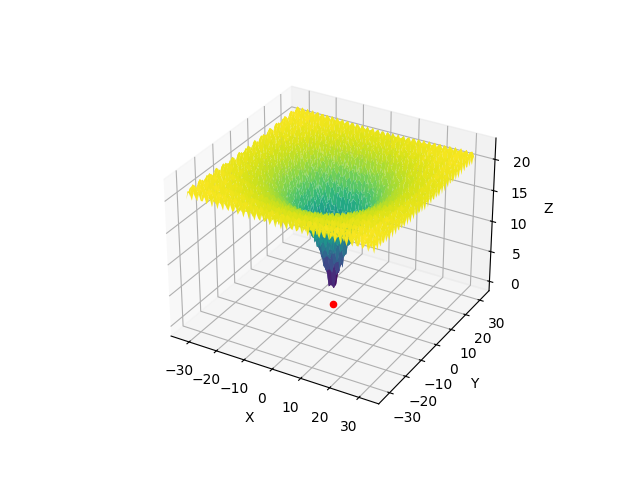
\includegraphics[width=\textwidth]{images/ackley_3d.png}
        \caption{Ackley function (3D).}
        \label{fig:ackley_3d}
    \end{subfigure}
    \hfill
    \begin{subfigure}[b]{0.45\textwidth}
        \centering
        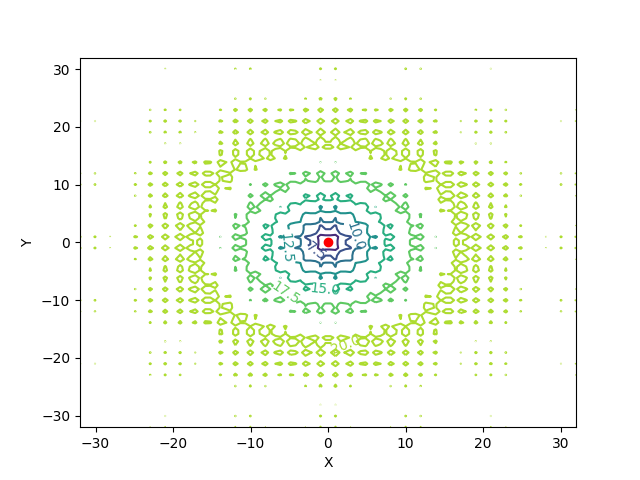
\includegraphics[width=\textwidth]{images/ackley_contour.png}
        \caption{Ackley function (Contour).}
        \label{fig:ackley_contour}
    \end{subfigure}
    \caption{Ackley function visualizations.}
    \label{fig:ackley}
\end{figure}

\begin{figure}[h!]
    \centering
    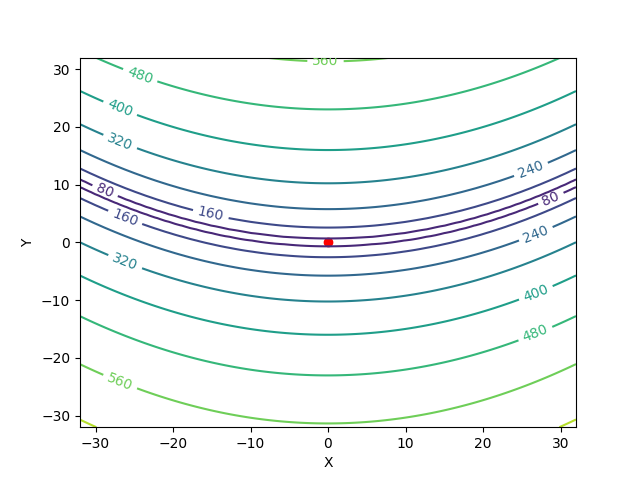
\includegraphics[width=0.45\textwidth]{images/bukin_function_n6_contour.png}
    \caption{Bukin Function N.6.}
    \label{fig:bukin}
\end{figure}

\begin{figure}[h!]
    \centering
    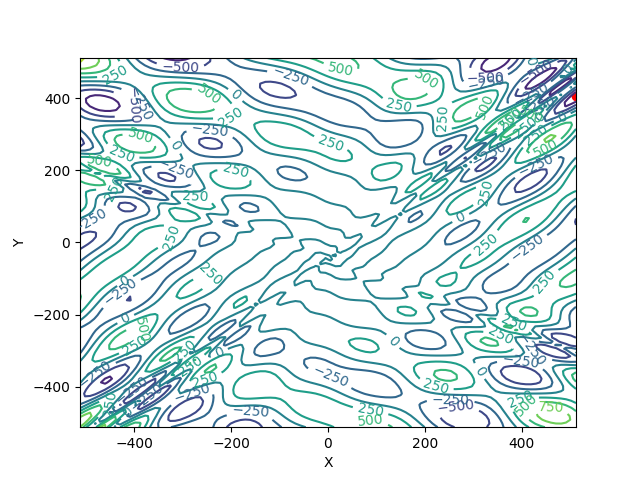
\includegraphics[width=0.45\textwidth]{images/eggholder_function_contour.png}
    \caption{Eggholder function.}
    \label{fig:eggholder}
\end{figure}

\begin{figure}[h!]
    \centering
    \begin{subfigure}[b]{0.45\textwidth}
        \centering
        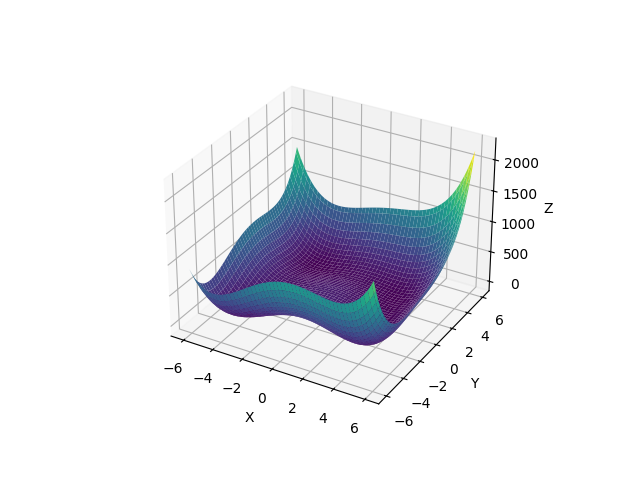
\includegraphics[width=\textwidth]{images/himmelblau_3d.png}
        \caption{Himmelblau function (3D).}
        \label{fig:himmelblau_3d}
    \end{subfigure}
    \hfill
    \begin{subfigure}[b]{0.45\textwidth}
        \centering
        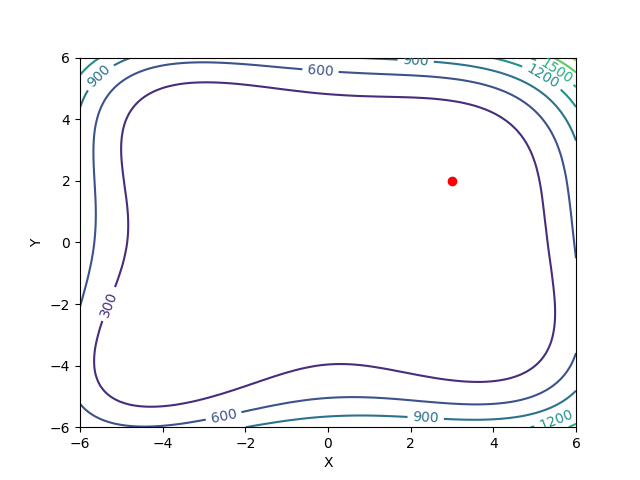
\includegraphics[width=\textwidth]{images/himmelblau_contour.png}
        \caption{Himmelblau function (Contour).}
        \label{fig:himmelblau_contour}
    \end{subfigure}
    \caption{Himmelblau function visualizations.}
    \label{fig:himmelblau}
\end{figure}

\newpage

\section{Результаты}
\subsection{Графики сходимости}
Графики сходимости SWO на различных тестовых функциях представлены на Рисунке \ref{fig:convergence}.

\begin{figure}[h!]
    \centering
    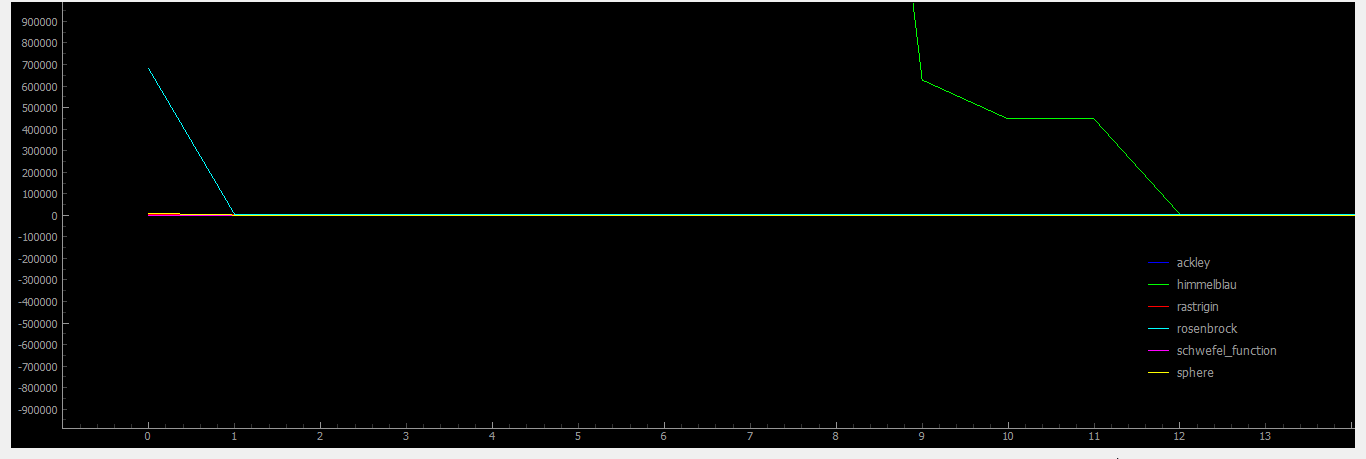
\includegraphics[width=1.2\textwidth]{images/convergence_GUI.png}
    \caption{Сходимость SWO на тестовых функциях.}
    \label{fig:convergence}
\end{figure}

\subsection{Результаты оптимизации}
Результаты оптимизации для различных тестовых функций представлены в таблице \ref{tab:results}.

\begin{table}[h!]
\centering
\begin{tabular}{@{}lllll@{}}
\toprule
Функция & Оптимальное значение (fmin) & Оптимальное решение (xmin) & Общее количество оценок (neval) & Оценки для функции \\
\midrule
Sphere & $1.70 \times 10^{-59}$ & $[-3.69 \times 10^{-30}, 1.85 \times 10^{-30}]$ & 9225 & 9225 \\
Ackley & $-4.44 \times 10^{-16}$ & $[-3.68 \times 10^{-18}, -1.71 \times 10^{-16}]$ & 13585 & 13585 \\
Bukin N.6 & $1.00 \times 10^{-1}$ & $[2.34 \times 10^{-19}, 4.83 \times 10^{-25}]$ & 17145 & 17145 \\
Eggholder & $-894.58$ & $[-465.69, 385.72]$ & 12445 & 12445 \\
Himmelblau & $4.93 \times 10^{-17}$ & $[-2.81, 3.13]$ & 18145 & 18145 \\
Rastrigin & $0.0$ & $[7.67 \times 10^{-10}, -4.84 \times 10^{-10}]$ & 10925 & 10925 \\
Rosenbrock & $0.0$ & $[1.0, 1.0]$ & 16805 & 16805 \\
Schwefel & $2.55 \times 10^{-5}$ & $[420.97, 420.97]$ & 13085 & 13085 \\
\bottomrule
\end{tabular}
\caption{Результаты оптимизации для различных тестовых функций.}
\label{tab:results}
\end{table}


\newpage

\section{Заключение}
Spider Wasp Optimizer демонстрирует высокую эффективность при решении задач оптимизации. Алгоритм успешно протестирован на различных тестовых функциях. Будущие работы направлены на улучшение адаптивности алгоритма, а также его применение в реальных задачах.

\end{document}
